\documentclass{article}
\usepackage[utf8]{inputenc}
\usepackage{cite}
\usepackage{amsmath,amssymb,amsfonts}
\usepackage{algorithmic}
\usepackage{graphicx}
\usepackage{textcomp}
\usepackage{xcolor}
\usepackage{textgreek}
\usepackage{multicol}
\usepackage{lipsum}
\usepackage{mwe}
\usepackage{outlines}
\usepackage{subcaption}
\usepackage{enumitem}
\usepackage[toc,page]{appendix}
\setlist[enumerate]{label*=\arabic*.}
\usepackage[]{algorithm2e}

\usepackage[a4paper, total={6in, 9in}]{geometry}

\begin{document}

\begin{titlepage}
   \begin{center}
      \vspace*{1cm}

       \textbf{Industrial Automation - Project 1}

      \vspace{0.5cm}
        Sampling Theory and Reconstruction
            
       \vspace{1.5cm}

       \textbf{Arpit Savarkar}
        
                % \begin{figure}[htbp]
                %     \begin{center}
                % 	\includegraphics[width=70mm]{figures/Complete_Assembly.jpg}
                %     \end{center}
                % \end{figure}
            
            
   \end{center}
\end{titlepage}

\section{Abstract}
Digital hardware, from micro-controllers to super computers, perform and analyze actions in discrete steps. They cannot directly handle the continuous-timer signals that are prevalent in the Newtonian Physical world. This report attempts at interfacing between these two worlds, one discrete, the other continuous. A discrete-time signal is constructed by sampling a continuous-time signal, and a continuous-time signal is reconstructed by interpolating a discrete-time signal. \cite{b7}

% https://cnx.org/contents/d2CEAGW5@15.4:IWHZ6hxG@13/Discrete-Time-Processing-of-Continuous-Time-Signals

\section{Introduction}
Original continuous time signal \textit{\textbf{x}} is sampled to a discrete time signal $ x_s $ in such a way that the periods of the samples spectrum $ X_s $ is as close as possible in shape to the spectrum of X. Then a discrete time, linear time invariant filter is applied, which modifies the shape of the samples spectrum but cannot increase the bandlimit to produce another signal. This is reconstructed with a suitable reconstruction filter to produce a continuous time output signal thus effectively implementing some continuous time system. 

\begin{figure}[htbp]
    \begin{center}
    	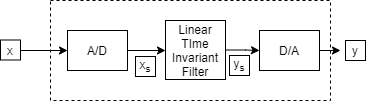
\includegraphics[width=100mm, angle=0,rotate=0]{figures/adc_dac (1).png}
    \end{center}
        \caption{Digital Signal Processing (Short)}
\end{figure}

The analog to digital converter, often denoted by ADC or A/D. It is clear that in order to process a continuous time signal using discrete time techniques, we must sample the signal as an initial step. This is essentially the purpose of the ADC, although there are practical issues that which will be discussed later. An ADC takes a continuous time analog signal as input and produces a discrete time digital signal as output, with the ideal infinite precision case corresponding to sampling. As per Nyquist-Shannon Sampling theorem, in order to retain all information about the original signal, we usually wish sample above the Nyquist frequency. 

The discrete time filter is where the intentional modifications to the signal information occur. This is commonly done in digital computer software after the signal has been sampled by a hardware ADC and before it is used by a hardware DAC to construct the output. Any modifications that the discrete filter makes to this shape can be passed on to a continuous time signal assuming perfect reconstruction. Consequently, the process described will implement a continuous time, linear time invariant filter.


\begin{figure}[htbp]
    \begin{center}
    	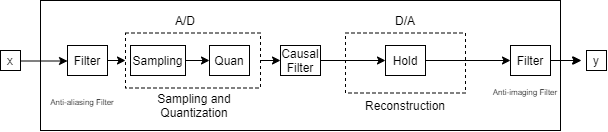
\includegraphics[width=100mm, angle=0,rotate=0]{figures/adc_dac_complete.png}
    \end{center}
        \caption{Digital Signal Processing - Detailed}
\end{figure}

\subsubsection{Signal Quantization}
In our preceding discussion of discrete time processing of continuous time signals, we had assumed an ideal case in which the ADC performs sampling exactly. However, while an ADC does convert a continuous time signal to a discrete time signal, it also must convert analog values to digital values for use in a digital logic device, a phenomenon called quantization. 

\subsubsection{Filter Implementability}
In real world circumstances, if the input signal is a function of time, the future values of the signal cannot be used to calculate the output. Thus, the digital filter and the overall system must be causal. If the desired system is not causal but has impulse response equal to zero before some time t0, a delay can be introduced to make it causal. However, if this delay is excessive or the impulse response has infinite length, a windowing scheme becomes necessary in order to practically solve the problem. 

Take, for instance the case of the ideal lowpass filter. It is acausal and infinite in length in both directions. Thus, we must satisfy ourselves with an approximation. One might suggest that these approximations could be achieved by truncating the sinc impulse response of the lowpass filter at one of its zeros, effectively windowing it with a rectangular pulse. However, doing so would produce poor results in the frequency domain as the resulting convolution would significantly spread the signal energy. Other windowing functions, of which there are many, spread the signal less in the frequency domain and are thus much more useful for producing these approximations.

\section{Mathematical Background}

\subsection{Fourier series}
Fourier series are infinite series that represent periodic functions in terms of cosines and sines. A signal f(x) is called a periodic function if f(x) is defined for all real x, except possibly at some points, and if there is some positive number p, called a period of , such that
\begin{equation}
\begin{aligned}
     f (x + n.p) = f (x)
\end{aligned}
\label{eq:periodic_function}
\end{equation}

The particular conditions that a function f(x) must fulfil in order that it may be expanded as a Fourier series are known as the Dirichlet conditions, and may be summarised by
the following four points:

\begin{enumerate}
    \item
    The function must be periodic
    
    \item
    It must be single-valued and continuous, except possibly at a finite number of finite discontinuities
    
    \item 
    It must have only a finite number of maxima and minima within one period;
    
    \item
    The integral over one period of |f(x)| must converge
\end{enumerate}

Fourier series simply states that, periodic signals can be represented into sum of sines and cosines when multiplied with a certain weight.In hindsight it shows that periodic signals can be broken down into further signals. 

\begin{equation}
\begin{aligned}
     f(x) = a_0 + \Sigma(a_n cos(n.x) + b_n sin(n.x))
\end{aligned}
\label{eq:fourier_Series}
\end{equation}

\eqref{eq:fourier_Series} is called the fourier series of f(x). 

As a Fourier series expansion in general contains both sine and cosine parts, it may be written more compactly using a complex exponential expansion. This simplification makes use of the property that $exp(jrx) = cosrx + i sin rx$. The complex Fourier series expansion is written as
\begin{equation}
\begin{aligned}
     f(x) = \Sigma c_r e^{j.\omega.x}
\end{aligned}
\label{eq:complex_fourier_Series}
\end{equation}

where the Fourier coefficients are given by 
\begin{equation}
\begin{aligned}
     f(x) = 1/T_0 \int_{x_0}^{x_0 + T} f(x) e^{j.\omega.t} . dx
\end{aligned}
\label{eq:coeff_complex_fourier_Series}
\end{equation}

\subsection{Fourier Transforms}
The Fourier transform provides a representation of functions defined over an infinite interval and having no particular periodicity, in terms of a superposition of sinusoidal functions. It may thus be considered as a generalisation of the Fourier series representation of periodic functions. In order to develop the transition from Fourier series to Fourier transforms, we first recall that a function of period T may be represented as a complex Fourier series as 

\begin{equation}
\begin{aligned}
     f(t) = \Sigma_{r = -\infty}^{\infty} c_r e^{j.\omega_r.t}
\end{aligned}
\label{eq:complex_1}
\end{equation}

\begin{figure}[htbp]
        \begin{center}
    	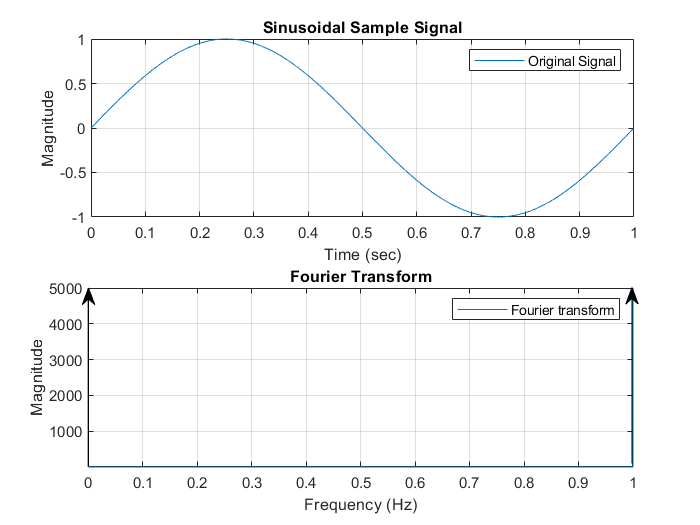
\includegraphics[width=100mm, angle=0,rotate=0]{figures/Fourier_Transform.png}
        \end{center}
        \caption{Fourier Transform of Sine Wave}
\end{figure}

As the period T tends to infinity, the ‘frequency quantum' $\Delta \omega$ becomes vanishingly small and the spectrum of allowed frequencies $\omega.r$ becomes a continuum. Thus, the infinite sum of terms in the Fourier series becomes an integral, and the coefficients $c_r$ become functions of the continuous variable $\omega$

\begin{equation}
\begin{aligned}
     c_r = 1/T \int_{-T/2}^{T/2} f(t) * e^{-j.\omega_k t} . dt
\end{aligned}
\label{eq:complex_2}
\end{equation}

where we have written the integral in two alternative forms and, for convenience, made one period run from − T/2 to +T/2 rather than from 0 to T. Substituting eq \eqref{eq:complex_2} in \eqref{eq:complex_1} gives us 
\begin{equation}
\begin{aligned}
     f(t) = \Sigma_{r = -\infty}^{\infty} \frac{\Delta\omega}{2.\pi} \int_{-T/2}^{T/2} f(u).e^{-j\omega_k.u} du . e^{j\omega_k.u} 
\end{aligned}
\label{eq:complex_3}
\end{equation}

If T tends to $\infty$ then $\Delta \omega = 2π/T $ becomes infinitesimal, the width of the rectangles tends to zero and, from the mathematical definition of an integral,
\begin{equation}
\begin{aligned}
     f(\omega_k) = \int_{-\infty}^{\infty} f(\omega)*e^{j.\omega.t} d\omega
\end{aligned}
\label{eq:complex_4}
\end{equation}

And the continuous time Fourier transform of X(t) becomes 
$c_k$ = $\int_{-\infty}^{\infty} X(t) e^{-j.\omega_k . dt}$

\subsubsection{Relation of dirac delta function to Fourier Transforms}
Dirac $\delta$-function as a way of representing
very sharp narrow pulses. By Fourier inversion theorem
\begin{equation}
\begin{aligned}
     X(t) = \frac{1}{2.\pi} \int_{-\infty}^{\infty} d\omega e^{j.\omega.t} \int_{-\infty}^{\infty} du X(u) e^{-j.\omega.u} \\
     
     = \int_{-\infty}^{\infty} du X(u) \{ \frac{1}{2.\pi} \int_{-\infty}^{\infty} e^{j.\omega.(t-u) } d\omega \}
\end{aligned}
\label{eq:complex_5}
\end{equation}

The Dirac $\delta$-function has the property that $\delta(t) = 0 \ for \ t \neq 0$
but the fundamental defining property is 
\begin{equation}
\begin{aligned}
     \int X(t)\delta(t-a) dt = X(a)
\end{aligned}
\label{eq:dirac_property}
\end{equation}

provided the range of integration includes the point t = a; otherwise the integral equals zero.
\begin{equation}
\begin{aligned}
    \implies \delta(t-u) = 1/T \int_{-\infty}^{\infty} e^{j.\omega.(t-u) d\omega}
\end{aligned}
\end{equation}

Considered as a Fourier transform, this representation shows that a very narrow time peak at t = u results from the superposition of a complete spectrum of harmonic waves, all frequencies having the same amplitude and all waves being in phase at t = u. This suggests that the $delta$-function may also be represented as the limit of the transform of a uniform distribution of unit height as the width of this distribution becomes infinite.

\section{Sampling}

% Reference: https://ptolemy.berkeley.edu/projects/chess/eecs124/reading/LeeAndVaraiya11.pdf

\subsection{Introduction}
\cite{b6} A sampler for complex-valued signals is a system 
\begin{equation}
\begin{aligned}
    Sampler_T:[Reals->Complex] -> [Integers -> Complex],
\end{aligned}
\end{equation}
where T is the sampling interval (units seconds/sample). The sampling frequency or sample rate is $f_s$ = 1/T (in units of samples/second or Hz) or $\omega_s = 2.\pi / T$, in units of radians/second. 
\begin{equation}
\begin{aligned}
    y[n] = x[nT]
\end{aligned}
\end{equation}

% https://neuron.eng.wayne.edu/auth/ece4330/lectures/lecture_23_ece4330t.pdf
\cite{b5} Discrete-time system implementation  takes advantage of the flexibility and efficiency of digital processors. A sequence X[n] can be obtained from a
continuous-time signal X(t) through sampling. Here, the value of X[n] for some integer n is equal to X(n$T_s$), the value of X(t) at time t = (n$T_s$). So,
we sample at regular intervals of width $T_s$ seconds or 1/$T_s$ hz.  It is kind of intuitive to argue that sampling generally leads to loss of signal information. 

\subsection{The sampling process}
Sampling in theory, consists of simply modulating the signal by another signal, $\delta(t)$, which consists of a train of unit-impulses separated by $T_s$ seconds (Dirac delta property \eqref{eq:dirac_property}).

\begin{equation}
\begin{aligned}
    X_s(t) = X(t).\delta_s(t) = X(t) \Sigma_{n = -\infty}^{\infty} \delta(t-n.T_s) 
\end{aligned}
\end{equation}

\begin{equation}
\begin{aligned}
    \implies X_s(t) =  \Sigma_{n = -\infty}^{\infty} X(n.T_s). \delta(t-n.T_s)
\end{aligned}
\end{equation}

Considering the frequency domain. By frequency convolution property  
\begin{equation}
\begin{aligned}
    \delta_s(t) =  \Sigma_{n = -\infty}^{\infty} \delta(t - n.T_s) \\
     = \frac{1}{T_s} \Sigma_{n = -\infty}^{\infty} e^{j.n.\omega_s.t} \\
     = \frac{\omega_s}{2.\pi} \Sigma_{n = -\infty}^{\infty} e^{j.n.\omega_s.t}
\end{aligned}
\end{equation}

By Fourier Pair property and superposition principle 
\begin{equation}
\begin{aligned}
    F \{ \delta_s(t) \} = \omega_s \Sigma_{n = -\infty}^{\infty} \delta(\omega - n\omega_s 
\end{aligned}
\end{equation}

From the impulse train analysis eq 14, where f and $f_s$ are the frequencies of the signal under consideration
\begin{equation}
\begin{aligned}
    X(f) = \Sigma_{n = -\infty}^{\infty} f_s . F(f-n.f_s)
\end{aligned}
\end{equation}

The above equation represents a very important and elegant result. It states that, in the frequency domain, the sampled signal is essentially a superposition of shifted  (by integer multiples of the sampling frequency, $f_s$. versions of the spectrum of the signal f(t). 

% INSERT A FIGURE HERE ABOUT SIGNAL REPEATING
Figure shows that if the sampling frequency $f_s$ is twice the bandwidth of the bandlimited signal X(t). then the there will be no overlap between fourier transform of the time doamin signal and its its images, therefore an ideal low-pass fikter with a cutoff frequency of $f_o = \frac{f_s}{2}$ and a DC gain of $T_s$ can be used to perfectly reconstruct X(t). 

\begin{figure}[htbp]
    \begin{center}
	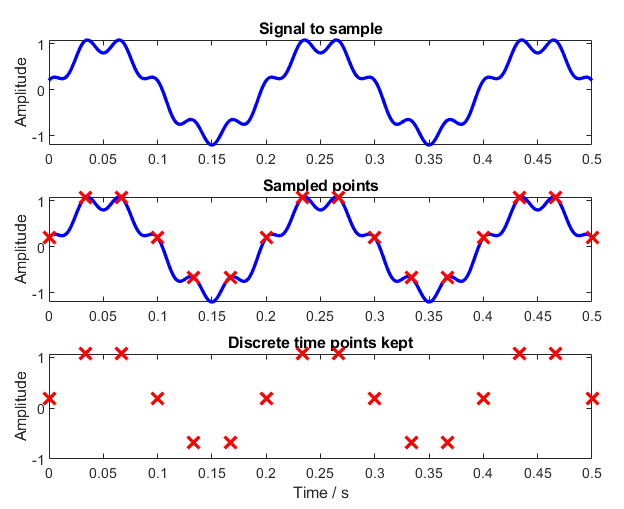
\includegraphics[width=80mm]{figures/Sampling_in_process.PNG}
    \end{center}
    \caption{Sampling in Progress}
\end{figure}

Frequency Domain for a simple pulse of the input signal looks (with brevity of zooming in) as seen in Figure 5. 

\begin{figure}[htbp]
    \begin{center}
	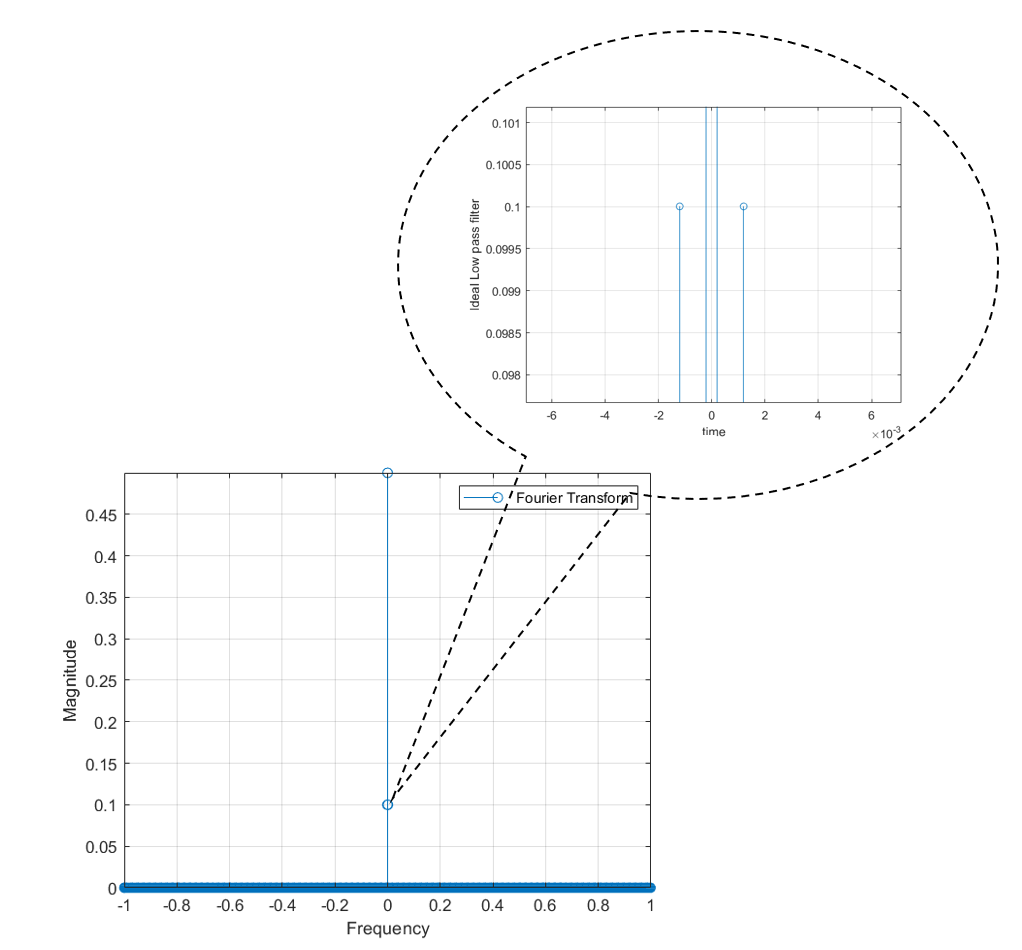
\includegraphics[width=85mm]{figures/Main_f.png}
    \end{center}
    \caption{Frequency Spectrum for a single impulse}
\end{figure}

\subsubsection{Sampling and Frequency Domain experiment }

\begin{enumerate}

    \item An impulse at the sine frequency (blue). The Fourier transform of a sine of frequency f is an impulse at frequencies f and -f.
    
    \item A copy of the above, but centered around the sampling frequency rather than 0 Hz (red).
    
    \item A copy of around 2 degree the sampling frequency in magentia. This continues, but higher harmonics are not plotted here.
\end{enumerate}


The signal that we want is the one in blue occurring between 0 and 2.$ \omega_{max} $ the sampling frequency (vertical black line). If the sampling rate is too low, or the signal frequency too high, other components enter this zone (between zero and the black line). When this happens the output will a very low frequency sine, not the one we sampled. Which is aliasing. 

\begin{figure}[!htb]
    \minipage{0.5\textwidth}
      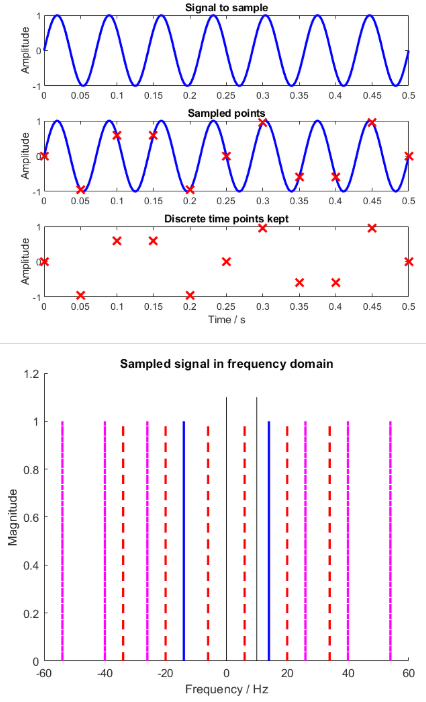
\includegraphics[width=6cm, height=8cm, angle=0,rotate=0]{figures/Sample_Sinusoidal.PNG}
    \endminipage\hfill
    \minipage{0.5\textwidth}
      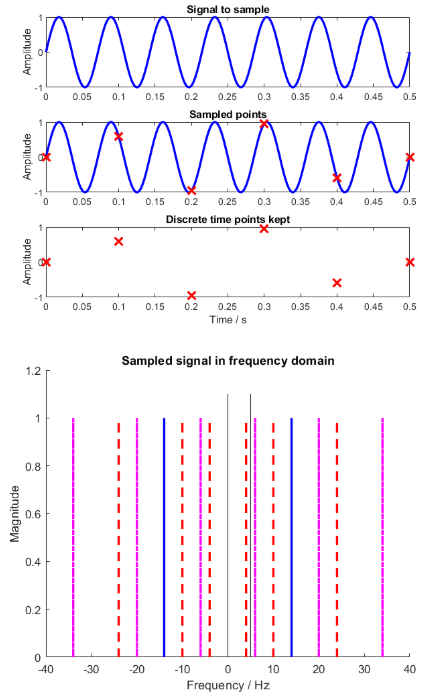
\includegraphics[width=6cm, height=8cm, angle=0,rotate=0]{figures/Sample_Sinusoidal_with_alias.PNG}
    \endminipage\hfill
    \caption{Sampling of input sample signal at multiple frequencies}
    \label{fig:Aliasing}
\end{figure}


\subsubsection{Nyquist-Shannon sampling theorem}
Let X(t) be a complex valued, continuous-time, band-limited signal with bandwidth B. And let X[n] be the sequence of numbers obtained by sampling X(t) at a sampling rate of $f_s$ Hz. Then X(t) can be perfectly reconstructed from its samples X[n], iff $ f_s > $ 2B. 

\begin{figure}[!htb]
    \minipage{0.33\textwidth}
      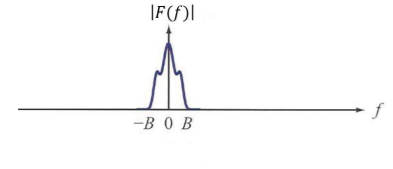
\includegraphics[width=5cm, height=3cm]{figures/Orig_Sample_Singal_Single_Impulse.PNG}
      \caption{Input Signal}
    \endminipage\hfill
    \minipage{0.33\textwidth}
      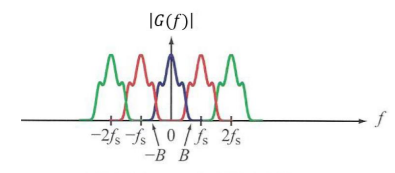
\includegraphics[width=5cm, height=3cm]{figures/Undersampled.PNG}
      \caption{Undersampled}
    \endminipage\hfill
    \minipage{0.33\textwidth}
      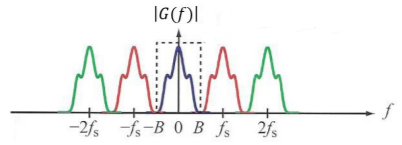
\includegraphics[width=5cm, height=3cm]{figures/Orig_Nyquiest.PNG}
      \caption{Nyquist Sampling}
    \endminipage\hfill
    \caption{Fourier Transform of repeated Pulse under variable sampling rate}
    \label{fig:shannon}
\end{figure}

Note how the magnitude spectrum |X(t)| is duplicated every $ f_s $ in the spectrum for |G(f)|. These duplicates are known as the image spectra. It shows that if the sampling frequency $ f_s $ is twice the bandwidth of the bandlimited signal X(t), then there will be no overlap between the spectras. therefore an ideal low-pass filter with a cut off frequency of $ f_o = \frac{f_s}{2} = B $ can be used perfectly. 

Increasing the sampling rate beyond 2B allows further separation between the images and its adjacent spectra, which showcases a more practical outset. On the other hand if we under sample, $ f_s < 2B $, then there will be overlap with the image spectra and the reconstructed signal will showcase signal in the reconstruction which were not part of the original signal. 

Consider \ref{fig:Aliasing}, showcases two different instances of sampling (magenta), and how if we undersample or oversample about the max frequency which is 14 Hz (Signal frequency) which get instances of magenta inside the black belt (ideal low pass - bandpass filter), which acts as the noise.

\begin{equation}
\begin{aligned}
    X(t) = X[n].sinc[\pi.f_s(t - nT_s)]
\end{aligned}
\end{equation}


\begin{figure}[!htb]
    \minipage{0.5\textwidth}
      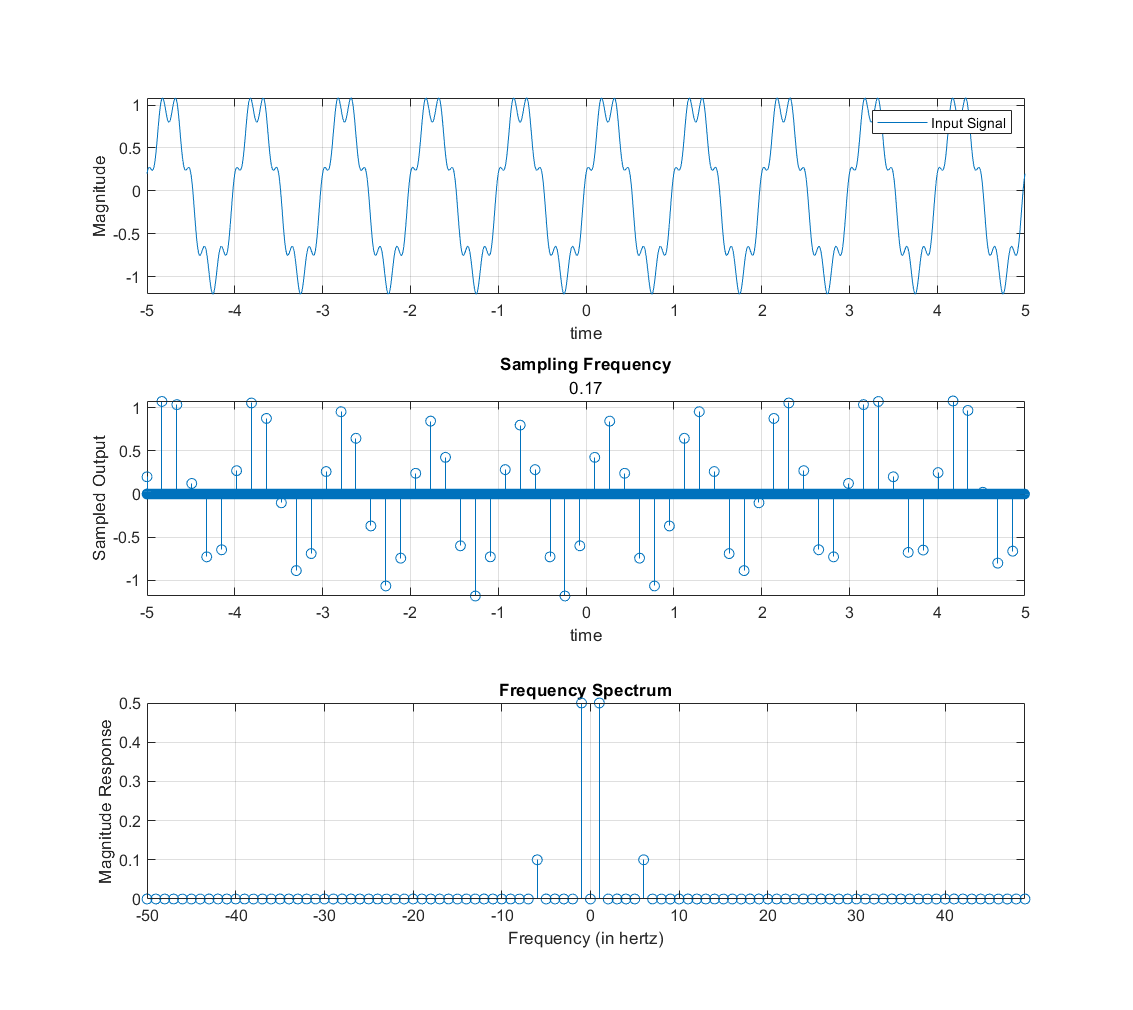
\includegraphics[width=8cm, height=8cm, angle=0,rotate=0]{figures/Input_Signal_0.17.png}
    \endminipage\hfill
    \minipage{0.5\textwidth}
      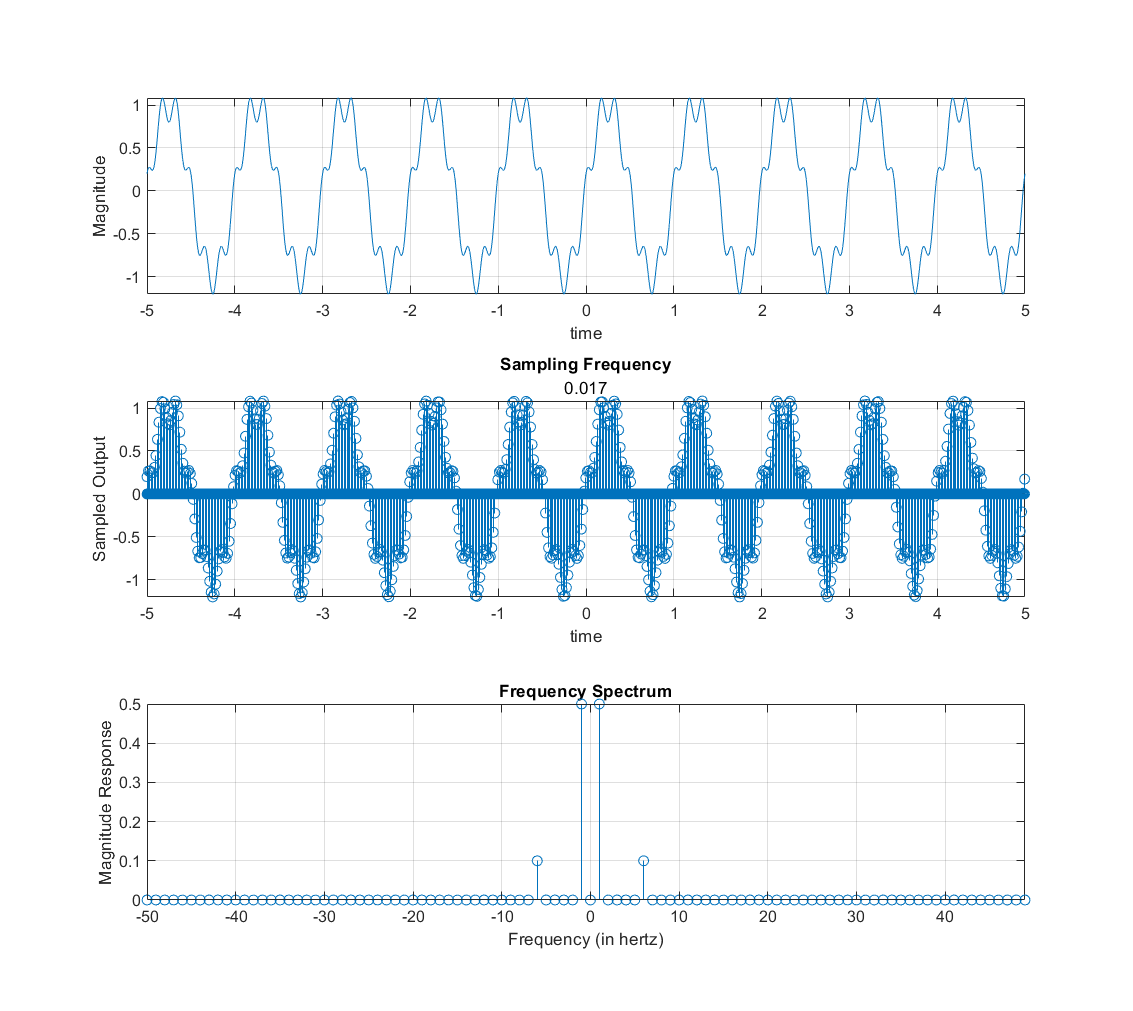
\includegraphics[width=8cm, height=8cm, angle=0,rotate=0]{figures/Input_Signal_0.017.png}
    \endminipage\hfill
    \caption{Sampling of given signal   }
\end{figure}



\section{Reconstruction}

The process of reconstructing a continuous time signal x(t) from its samples is known as interpolation. In the sampling theorem we saw that a signal x(t) band limited can be reconstructed from its samples. This reconstruction is accomplished by passing the sampled signal through a filter.  

In addition to bandlimited interpolation, a variety of other interpolation procedures are commonly used. One, referred to as a zero-order hold, interpolates between sample points by holding each sample value until the next sampling instant. This generates a staircase-like approximation to the original signal. Linear interpolation, also commonly referred to as a first-order hold, corresponds to connecting the sample points by straight line segments. Both the zero-order hold and first-order hold can be alternatively viewed in much the same way as we have discussed ideal bandlimited interpolation. Specifically, the zero-order hold corresponds to convolving the impulse train of samples with a rectangular pulse of duration exactly equal to the sampling period. The first-order hold corresponds to an impulse response for the reconstruction filter that is a triangle of duration equal to twice the sampling period. In the frequency domain, then, the zero-order hold corresponds to processing the samples with an approximation to a lowpass filter corresponding to the Fourier transform of a rectangular pulse. With the first-order hold the approximate lowpass filter has a frequency response that is the Fourier transform of a triangle.

In the frequency domain, the two-step process described above has a relatively straightforward interpretation. Through the process of sampling, assuming that the continuous-time signal is bandlimited and the conditions of the sampling theorem are met, the spectrum of the continuous-time signal is periodically replicated at integer multiples of the sampling frequency. Conversion of the impulse train to a discrete-time sequence corresponds in the time domain to a time normalization, in effect normalizing out the sampling period. Correspondingly, in the frequency domain, the frequency axis is normalized with the sampling frequency being scaled to a discrete-time frequency of $2 \pi $ . Thus, as we naturally expect, the Fourier transform of the discrete time sequence is periodic with a period of $2 \pi $. The periodicity can be interpreted as being a consequence of the basic sampling process. The normalization of the period in frequency to 27r is a consequence of the inherent time normalization in converting the impulse train of samples to a discrete time sequence.


\subsection{Ideal Low pass Filter}

\begin{equation}
\begin{aligned}
    X(\omega) = \int_{-\infty}^{\infty} x(t) e^{-j.\omega.t} dt \\
    = \int_{-\frac{T_0}{2}}^{\frac{T_0}{2}} l.e^{-j.\omega.t} dt \\
\end{aligned}
\end{equation}

\begin{equation}
\begin{aligned}
    X(\omega) = \frac{-1}{j.\omega} \left[e^{-j.\omega.t}\right]_{\frac{-To}{2}}^{\frac{To}{2}}
\end{aligned}
\end{equation}

\begin{equation}
\begin{aligned}
    X(\omega) = \frac{2}{\omega} sin(\frac{\omega.T}{2}) \\
    X(\omega) = T_o sinc(\frac{\omega.T_o}{2.\pi})
\end{aligned}
\end{equation}

    \begin{figure}[htbp]
        \begin{center}
    	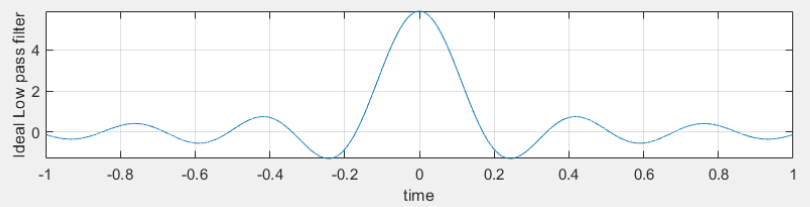
\includegraphics[width=100mm]{figures/sinc.PNG}
        \end{center}
        \caption{Ideal Low pass Filter in Time domain}
    \end{figure}
    
    \begin{figure}[!htb]
        \minipage{0.5\textwidth}
          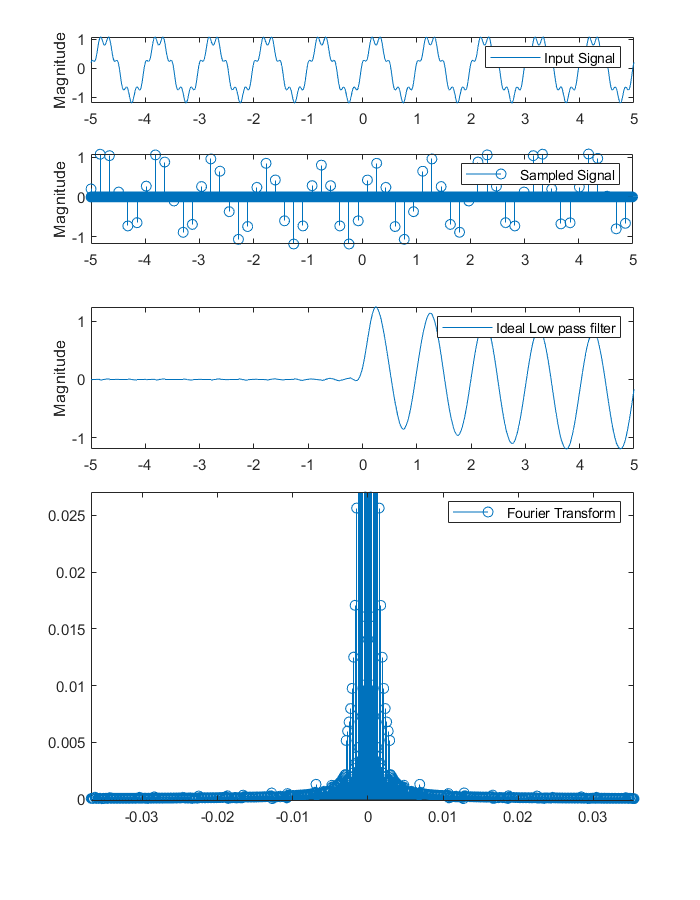
\includegraphics[width=8cm]{figures/Ideal_Low_Pass_Filter_0.17.png}
          \caption{Sampling Ts=0.17}
        \endminipage\hfill
        \minipage{0.5\textwidth}
          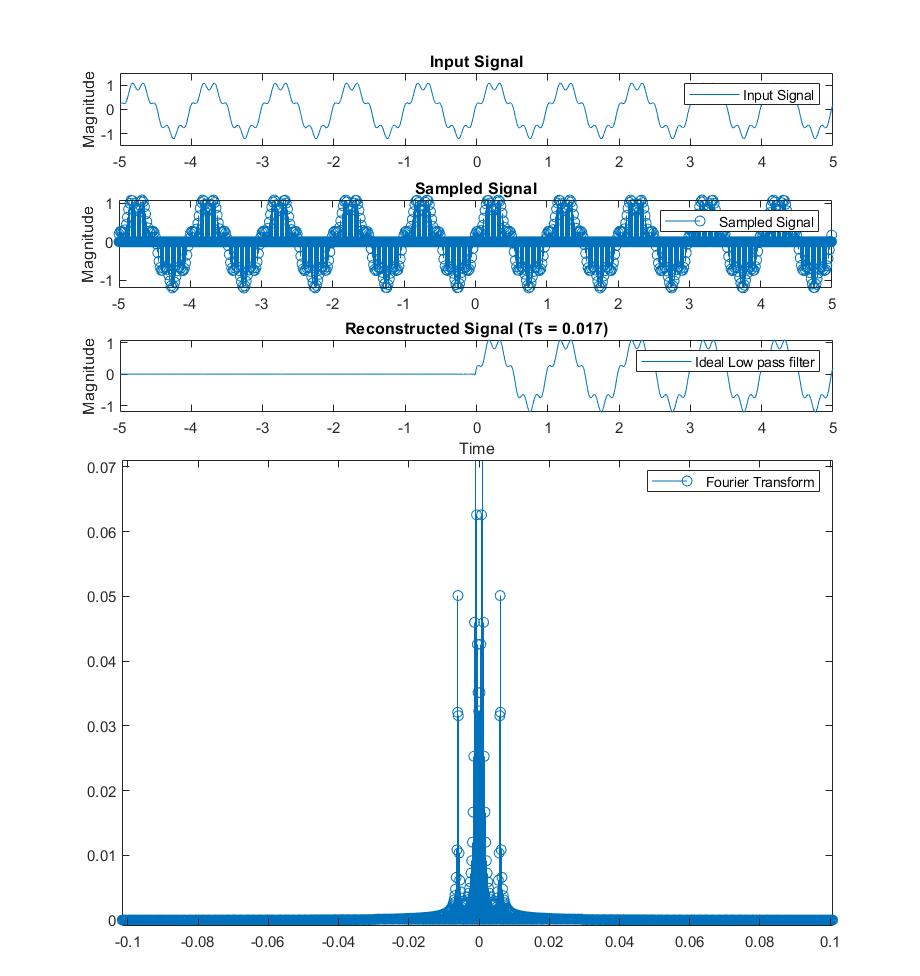
\includegraphics[width=8cm, height=9cm]{figures/Ideal_Low_Pass_Filter_0.017.png}
          \caption{Sampling Ts=0.017}
        \endminipage\hfill
        \caption{Signal Reconstruction - Low pass filter}
    \end{figure}

The description of the process of reconstruction in the frequency domain is to find the Discrete Fourier transform of the discrete time signal. 

Consider, the sinc function. To isolate the function indexed by k=0, we can multiply the Discrete fourier transform by a rectangle function that is wide enough to include the k = 0 alias but not wide enough to include any other aliases. So the corner of the rectangle must be at a value of F which is greater than Fm= fm/ fs, where fm is the highest frequency present in the signal x(t) but less than 1 - Fm or more compactly, $ Fm< Fc<1 - Fm$ . The isolated k = 0 replica is then

\begin{equation}
\begin{aligned}
    X(f) = rect(\frac{F}{F_c})  \Sigma_{n = -\infty}^{\infty} x[n] e^{-j.\omega.n}
\end{aligned}
\end{equation}

Undertaking, Inverse Fourier transform,

\begin{equation}
\begin{aligned}
    x(t) = F^{-1}(X(f)) 
\end{aligned}
\end{equation}


\begin{equation}
\begin{aligned}
     x(t) = \int_{-\infty}^{\infty} T rect((\frac{f}{f_s})/2Fc) \Sigma_{n = -\infty}^{\infty} x[n] e^{-j.\omega_n} e^{j.\omega_n} df
\end{aligned}
\end{equation}

By exchanging the order of integration and summation we can recognize the integrand as a time shifted inverse CTFT of a frequency domain rectangle function.

\begin{equation}
\begin{aligned}
    x(t) = T \Sigma_{n = -\infty}^{\infty} x[n] \int_{ -\infty}^{\infty} rect(\frac{f}{2f_c} e^{-j.\omega(t-nT)} df
\end{aligned}
\end{equation}

Then x[n] = x(nT) leads us, 

\begin{equation}
\begin{aligned}
    x(t) = 2(\frac{f_c}{f})  \Sigma_{n = -\infty}^{\infty} x(nT) sinc(2.f_c(t-nT))
\end{aligned}
\end{equation}

\cite{b3} The reconstruction process consists of replacing each sample by a sinc function, centered at the time of the sample and scaled by the sample value x(nT) times 2fc/ fs and adding all the functions so created. Suppose the signal is sampled at exactly Nyquist rate fs= 2fm, Then fm= fs/2 = fs- fm and Fm= 1/2 = 1- Fm.

The requirement $  Fm < Fc < 1- Fm $ cannot be met, in this case we must allow Fc= Fm, which means that fc= fm= fs/2 This will work till the signals spectrum does not have an impulse at fm. (If there is an impulse at fm , it will be aliased in the sampling process). In this limiting case, the interpolation is described by the simpler expression. Interpolation consists of simply of multiplying each sinc function by its corresponding sample value and then adding all the scaled and shifted sinc functions. 


\subsection{Zero Order Hold}
A continuous-time signal is often reconstructed by means of a device known as a zero-order hold, which simply maintains or holds the value x[n] for $ T_s $ seconds. The zero order hold is represented mathematically as a weighed sum of rectangular pulses shifted by integer multiples of the sampling interval. 

\begin{equation}
\begin{aligned}
    h_o(t) = \Big\{ 1, 0<t<T_s \\
             \Big\{ 0, t < 0, t > T_s
\end{aligned}
\end{equation}

Taking the Fourier transform, 
\begin{equation}
\begin{aligned}
    F \{ h_o(t) \} = 2.e^{-j.\omega.\frac{T_s}{2}} \frac{sin(\omega.Ts/2}{\omega} 
\end{aligned}
\end{equation}

That is, 
\begin{equation}
\begin{aligned}
    x_o(t) = h_o(t) * \Sigma_{n = -\infty}^{\infty} x[n]\delta(t-nTs) = h_o(t) * s_\delta (t)
\end{aligned}
\end{equation}

\begin{equation}
\begin{aligned}
    x_o(j.\omega) = H_o(j.\omega). X_\delta(j.\omega) 
\end{aligned}
\end{equation}

\begin{figure}[htbp]
    \begin{center}
	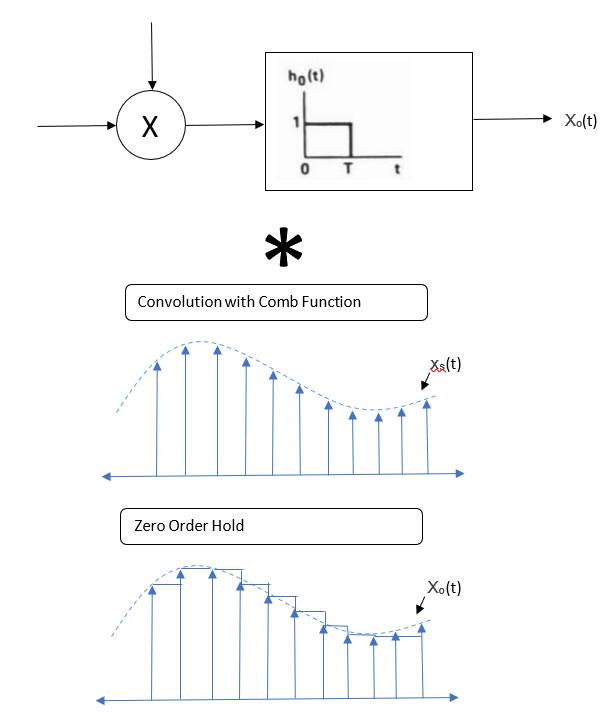
\includegraphics[width=5cm, height=6cm]{figures/ZOH.PNG}
    \end{center}
    \caption{Zero Order Hold Convolution}
\end{figure}

Comparing the input signal in the frequency domain, zero order hold introduces three modifications
\begin{itemize}
    \item A linear phase shift corresponding to a time delay of $ T_s / 2 $ sec. 
    
    \item 
    A distortion of portion of $ X_\delta (j.\omega) $ and attenuated , centered at nonzero multiples of $ \omega_s $
\end{itemize}

\begin{figure}[htbp]
    \begin{center}
	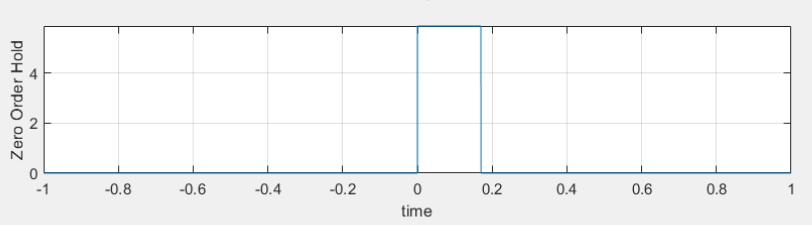
\includegraphics[width=80mm]{figures/ZOH_small.PNG}
    \end{center}
    \caption{Zero Order Hold in Time Domain}
\end{figure}


% Wikipedia : https://en.wikipedia.org/wiki/Zero-order_hold
\cite{b3} ZOH can also be modeled as the output of a linear time-invariant filter with impulse response equal to a rect function, and with input being a sequence of dirac impulses scaled to the sample values. The filter can then be analyzed in the frequency domain, for comparison with other reconstruction methods such as the Whittaker–Shannon interpolation formula suggested by the Nyquist–Shannon sampling theorem, or such as the first-order hold or linear interpolation between sample values.

In this method, a sequence of Dirac impulses, xs(t), representing the discrete samples, x[n], is low-pass filtered to recover a continuous-time signal, x(t).

Even though this is not what a DAC does in reality, the DAC output can be modeled by applying the hypothetical sequence of dirac impulses, xs(t), to a linear, time-invariant filter with such characteristics (which, for an LTI system, are fully described by the impulse response) so that each input impulse results in the correct constant pulse in the output.

    \begin{figure}[!htb]
        \minipage{0.5\textwidth}
          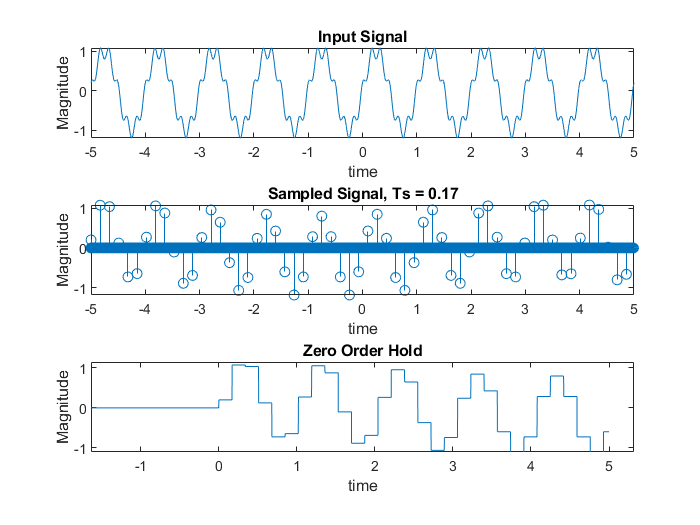
\includegraphics[width=8cm]{figures/Zero_Order_Hold_0.17.png}
          \caption{Sampling Ts=0.17}
        \endminipage\hfill
        \minipage{0.5\textwidth}
          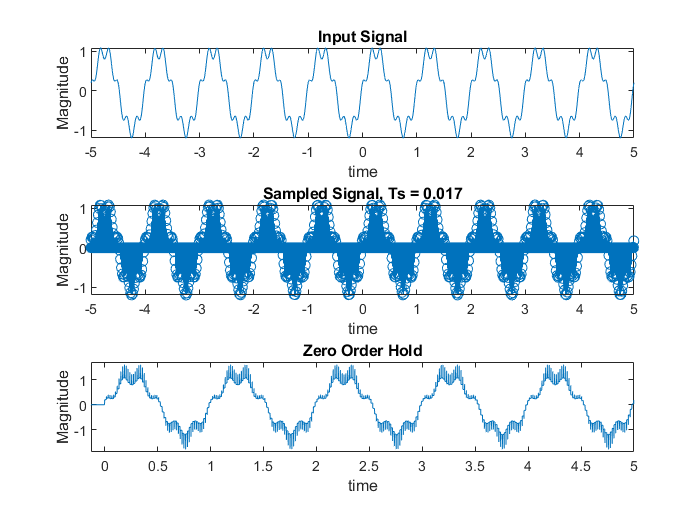
\includegraphics[width=8cm, height=9cm]{figures/Zero_Order_Hold_0.017.png}
          \caption{Sampling Ts=0.017}
        \endminipage\hfill
        \caption{Signal Reconstruction - Zero Order Hold}
    \end{figure}

\subsection{First Order Hold}
The First-Order Hold implements a first-order sample-and-hold that operates at the specified sampling interval.

\cite{b1} The first-order-hold (FOH) method is a mathematical model to reconstruct the sampled signals that could be done by a conventional digital-to-analog converter (DAC) and an analog circuit which is called an integrator. The FOH signal is reconfigured as a piecewise linear approximation of the original sampled signal. In [1], the FOH signal is used for real-time substructure testing, which is a novel method of testing structures under dynamic loading. An extrapolation of a first-order-hold discretization is used which increases the accuracy of the numerical model over more direct explicit methods. 

The first-order-hold (FOH)
is a better method to approximate the continuous analog signal than the zero-order hold
(ZOH)

From our previous analysis, the ideally sampled signal could be represented as

\begin{equation}
\begin{aligned}
    x_s(t) = T \Sigma_{n = -\infty}^{\infty} x(nT).\delta(t-nT)
\end{aligned}
\end{equation}

where x(t)is the original signal, $ x_s(t) $ is the ideal signal, $ \delta(t) $ is the Dirac impulse
function. Since a sequence of Dirac impulses, representing the discrete samples, is lowpass filtered, the mathematical model for FOH is necessary. The impracticality of
outputting a sequence of Dirac impulses foster the development of devices that use a
conventional DAC and some linear analog circuitry, to reconstruct the piecewise linear
output for the FOH signals.

The analytical piece-wise linear approximation 
\begin{equation}
\begin{aligned}
    x_{FOH}(t) = \Sigma_{n = -\infty}^{\infty} x(n.T) tri(\frac{t-nT}{T})
\end{aligned}
\end{equation}

where \textbf{tri} is the triangular function defined as, 
\begin{equation}
\begin{aligned}
    tri(t) = max(1-|t|, 0)
\end{aligned}
\end{equation}

However, the system represented by first order hold is not achievable in reality (non-causal). In fact, the typical FOH model used in practice is the delayed first-order hold, which is identical to the FOH except for the fact that its output is delayed by one sample period, resulting in a delayed piecewise linear output signal. 


\begin{figure}[htbp]
    \begin{center}
	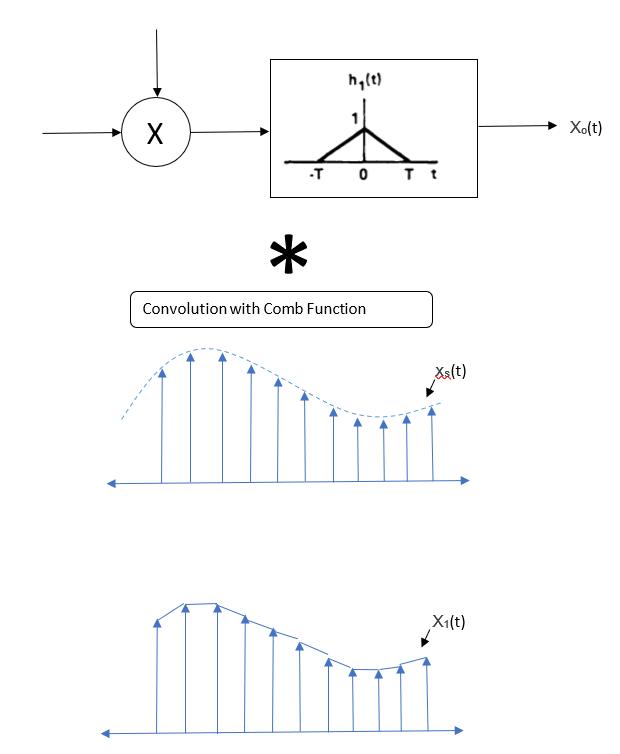
\includegraphics[width=80mm]{figures/FOH.PNG}
    \end{center}
    \caption{First Order Hold in Time Domain}
\end{figure}

Mathematical analysis of Fourier transform of a triangular pulse, considering the impulse from [-1 1]

\begin{equation}
\begin{aligned}
    F(tri(t)) = \int_{-\infty}^{\infty} tri(t) e^{-j.\omega.t} dt \\
    
    = \int_{-1}^{0} (1 + t)e^{-j.\omega.t} dt +  \int_{0}^{1} (1-t) (1-t)e^{-j.\omega.t}dt \\
    
    = -e^{-2.\pi.j.f}(e^{-2.\pi.j.f} -1)^2  \\
    
    = e^{-2.\pi.j.f}.e^{2.\pi.j.f}.4.j^2.sin(\pi.f)^2 * \frac{1}{4.\pi^2.f^2} \\
    
    = \sin(\pi.f) . \frac{1}{\pi.f} . \sin(\pi.f) . \frac{1}{\pi.f} \\
    
    = sinc^2 (f) \\
\end{aligned}
\end{equation}

\begin{figure}[!htb]
    \minipage{0.5\textwidth}
      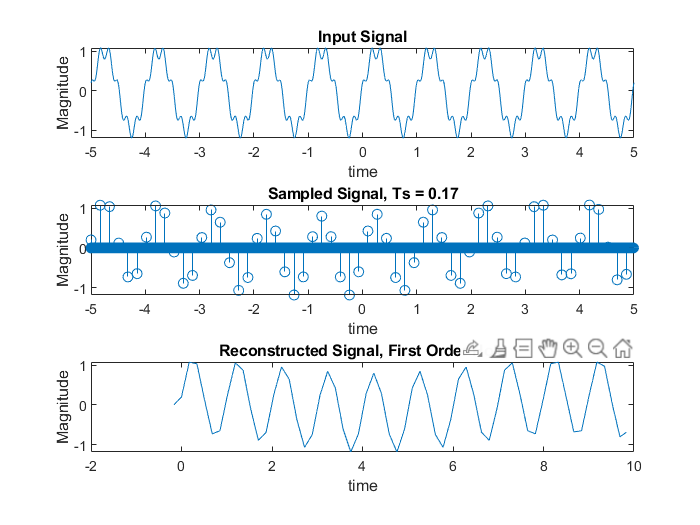
\includegraphics[width=8cm]{figures/First_Order_Hold_0.17.png}
      \caption{Sampling Ts=0.17}
    \endminipage\hfill
    \minipage{0.5\textwidth}
      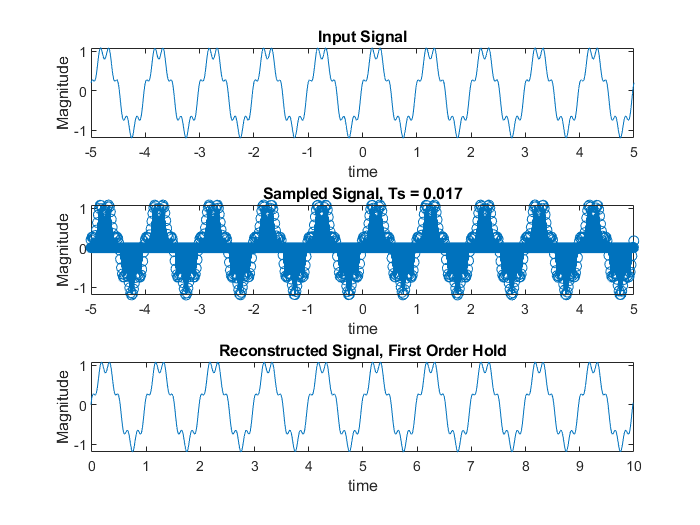
\includegraphics[width=8cm, height=9cm]{figures/First_Order_Hold_0.017.png}
      \caption{Sampling Ts=0.017}
    \endminipage\hfill
    \caption{Signal Reconstruction - First Order Hold}
\end{figure}
    

\begin{figure}[htbp]
    \begin{center}
	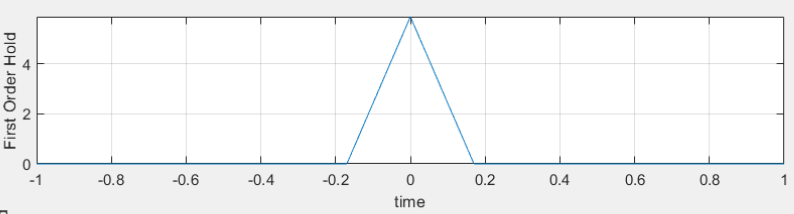
\includegraphics[width=80mm]{figures/FOH_.PNG}
    \end{center}
    \caption{First Order Hold}
\end{figure}    

    
\subsection{Predictive First-order hold}


\begin{figure}[htbp]
    \begin{center}
	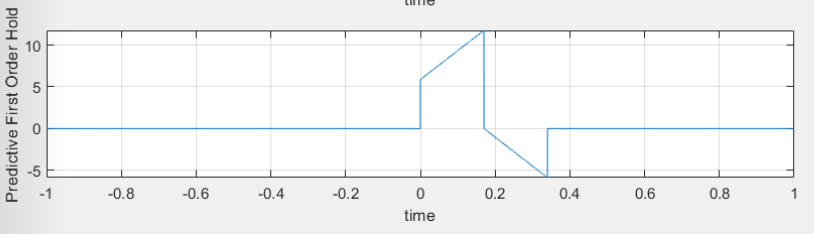
\includegraphics[width=80mm]{figures/PFOH.PNG}
    \end{center}
    \caption{Predictive First Order Hold}
\end{figure}

The predictive first-order hold is quite different. This is a causal hypothetical LTI system or filter that converts the ideally sampled signal into a piecewise linear output such that the current sample and immediately previous sample are used to linearly extrapolate up to the next sampling instance. The output of such a filter would be resulting in an effective impulse response of where rect(x) is the rectangular function and tri(x) is the triangular function. This a causal system. The impulse response of the predictive FOH does not respond before the input impulse. 
\\
Consider the input signal, 

\begin{equation}
\begin{aligned}
    x_s(t) = x(t) T \Sigma_{n = -\infty}^{\infty} \delta(t-nT) \\
    
    = T \Sigma_{n = -\infty}^{\infty} x(nT) \delta(t-nT)
\end{aligned}
\end{equation}


\begin{equation}
\begin{aligned}
    x_{FOH}(t) = \Sigma_{n = -\infty}^{\infty} (x(nT) + x(nT) - x((n-1)T)) \frac{t-nT}{T} rect(\frac{t-nT}{T} - 0.5)  )
    
    = \Sigma_{n = -\infty}^{\infty} x(nT) (\rect(t-nT)/T - 0.5 - rect(\frac{t-nT}{T}) - 1.5) + tri(\frac{t-nT}{T}-1)
\end{aligned}
\end{equation}
    
Taking the Fourier transform of the above response, 

\begin{equation}
\begin{aligned}
    F(h_{FOH}(t)) = (1 + j.\omega.T) {(\frac{1-e^{-j.\omega.T}}{j.\omega.T})}^2
\end{aligned}
\end{equation}
    
\begin{equation}
\begin{aligned}
    F(h_{FOH}(t)) = (1 + j.\omega.T) e^{-j.\omega.T} sinc(f.T)^2
\end{aligned}
\end{equation}

\begin{figure}[!htb]
    \minipage{0.5\textwidth}
      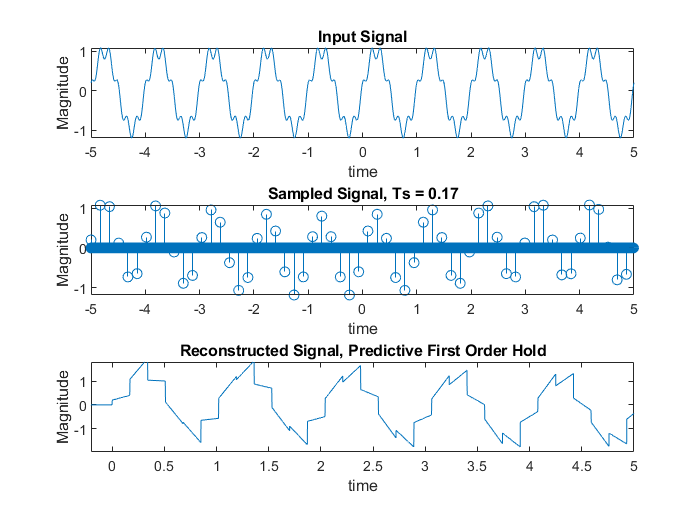
\includegraphics[width=8cm]{figures/Predictive_0.17.png}
      \caption{Sampling Ts=0.17}
    \endminipage\hfill
    \minipage{0.5\textwidth}
      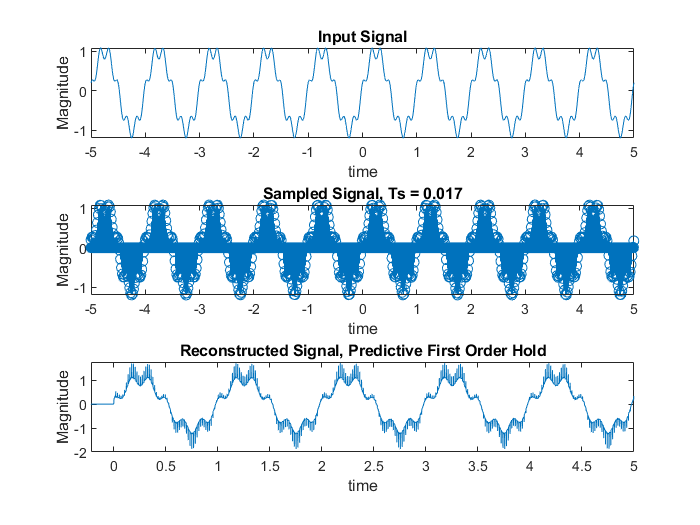
\includegraphics[width=8cm, height=9cm]{figures/Predictive_0.017.png}
      \caption{Sampling Ts=0.017}
    \endminipage\hfill
    \caption{Signal Reconstruction - Predicted First Order Hold}
\end{figure}

\subsection{Comparison of Fourier transforms of filters}

\begin{figure}[htbp]
    \begin{center}
	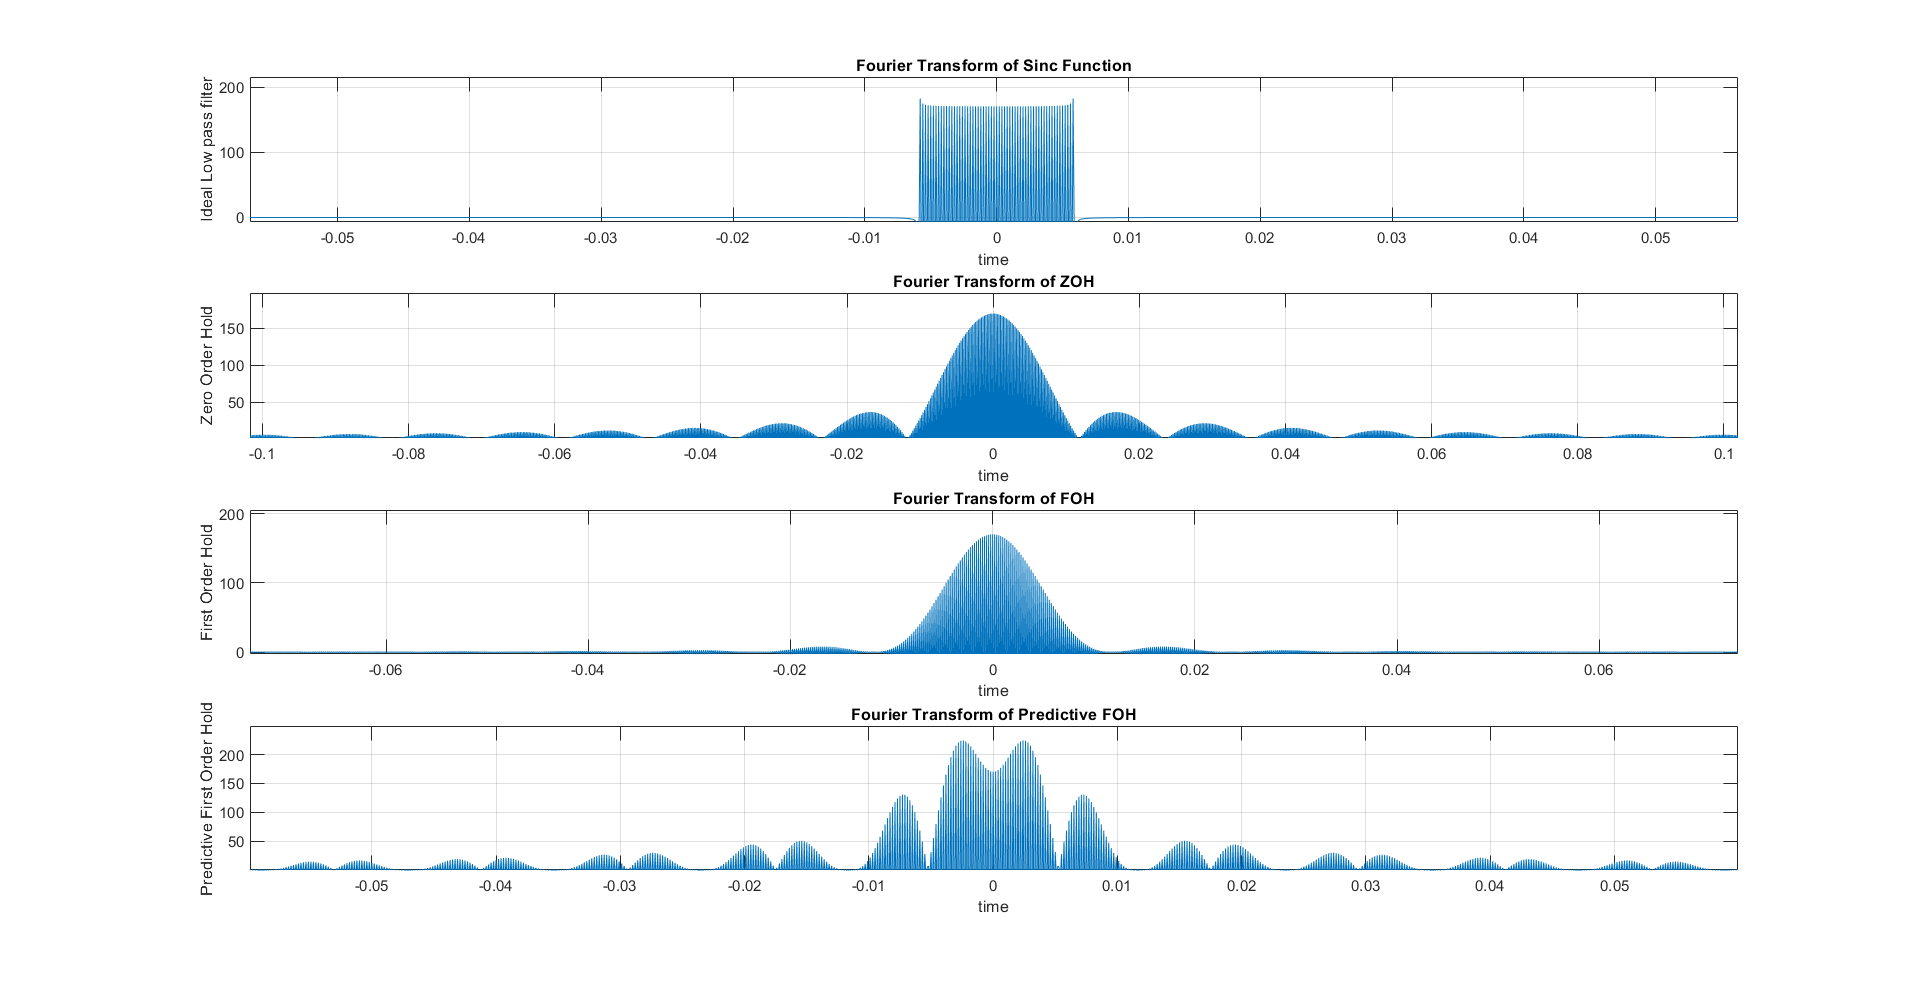
\includegraphics[width=175mm]{figures/Fourier_responses.png}
    \end{center}
    \caption{Fourier Responses}
    \label{fig:frfz}
\end{figure}

As can be seen \ref{fig:frfz}, the lobes of the magnitude for the first order leak out lesser magnitude at higher frequencies, thus forms a closer approximation after convolution to reconstruct a signal. The precision of first order hold in the discretization procedure combined with Taylor series expansion is higher than that of zero-order hold in most, though not all, situations. FOH and ZOH have their own advantages respectively for different input signals. FOH forms a more closer approximation. But is non-causal 

\subsection{Aliasing (or Spectral Folding)}
Because signals are not band-limited,  they have long tails in the frequency. 

% https://en.wikipedia.org/wiki/Aliasing#Folding
Aliasing \cite{b8} is an effect that causes different signals to become indistinguishable (or aliases of one another) when sampled. It also often refers to the distortion that results when a signal reconstructed from samples is different from the original continuous signal. 

Aliasing matters when one attempts to reconstruct the original waveform from its samples. The most common reconstruction technique produces the smallest of the $ f_N(f) $  frequencies. So it is usually important that $ f_0(f) $ be the unique minimum.  A necessary and sufficient condition for that is $ fs/2 > | f | $ ,  where $ fs/2 $ is commonly called the Nyquist frequency of a system that samples at rate  fs. 

When the condition $  fs/2 > f $  is met for the highest frequency component of the original signal, then it is met for all the frequency components, a condition called the Nyquist criterion. That is typically approximated by filtering the original signal to attenuate high frequency components before it is sampled. These attenuated high frequency components still generate low-frequency aliases, but typically at low enough amplitudes that they do not cause problems. A filter chosen in anticipation of a certain sample frequency is called an anti-aliasing filter.

The filtered signal can subsequently be reconstructed, by interpolation algorithms, without significant additional distortion. Most sampled signals are not simply stored and reconstructed. But the fidelity of a theoretical reconstruction (via the Whittaker–Shannon interpolation formula) is a customary measure of the effectiveness of sampling. 


\begin{figure}[htbp]
    \begin{center}
	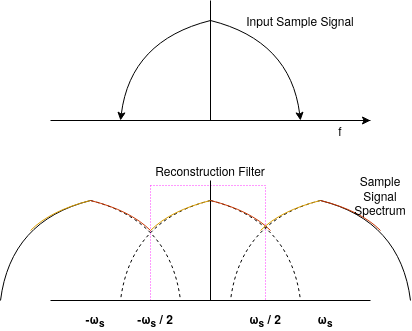
\includegraphics[width=100mm]{figures/Untitled Diagram.png}
    \end{center}
    \caption{Aliasing}
\end{figure}

\subsubsection{Anti-aliasing filter}

An \cite{b9} ideal anti-alias filter passes all the appropriate input frequencies (below f1) and cuts off all the undesired frequencies (above f1). However, such a filter is not physically realizable. In practice, filters look as shown in illustration. They pass all frequencies < f1, and cut-off all frequencies > f2. The region between f1 and f2 is known as the transition band, which contains a gradual attenuation of the input frequencies. \cite{b10} Although you want to pass only signals with frequencies < f1, those signals in the transition band could still cause aliasing. Therefore in practice, the sampling frequency should be greater than two times the highest frequency in the transition band. This turns out to be more than two times the maximum input frequency (f1). That is one reason why you may see that the sampling rate is more than twice the maximum input frequency.

But in comparison to a Fourier Transform of an ideal low pass filter which would lead to no leaks and would lead to perfect reconstruction. 

\begin{figure}[htbp]
    \begin{center}
	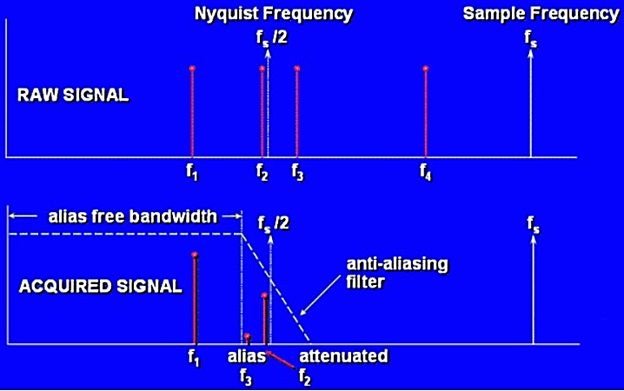
\includegraphics[width=80mm]{figures/anti_aliasing.png}
    \end{center}
    \caption{Aliasing Effect}
\end{figure}


\subsection{Reconstruction Conclusion}
Reconstruction \cite{b2} of a continuous time signal from a discrete time signal can be accomplished through several schemes. However, it is important that reconstruction is not the inverse of sampling and only produces one possible continuous time signal that samples to a given discrete time signal. As, perfect reconstruction of a bandlimited continuous time signal from its sampled version is possible using the Whittaker-Shannon reconstruction formula, which makes use of multiple filters under the condition that, if the sampling rate is sufficiently high.

\begin{figure}[htbp]
    \begin{center}
	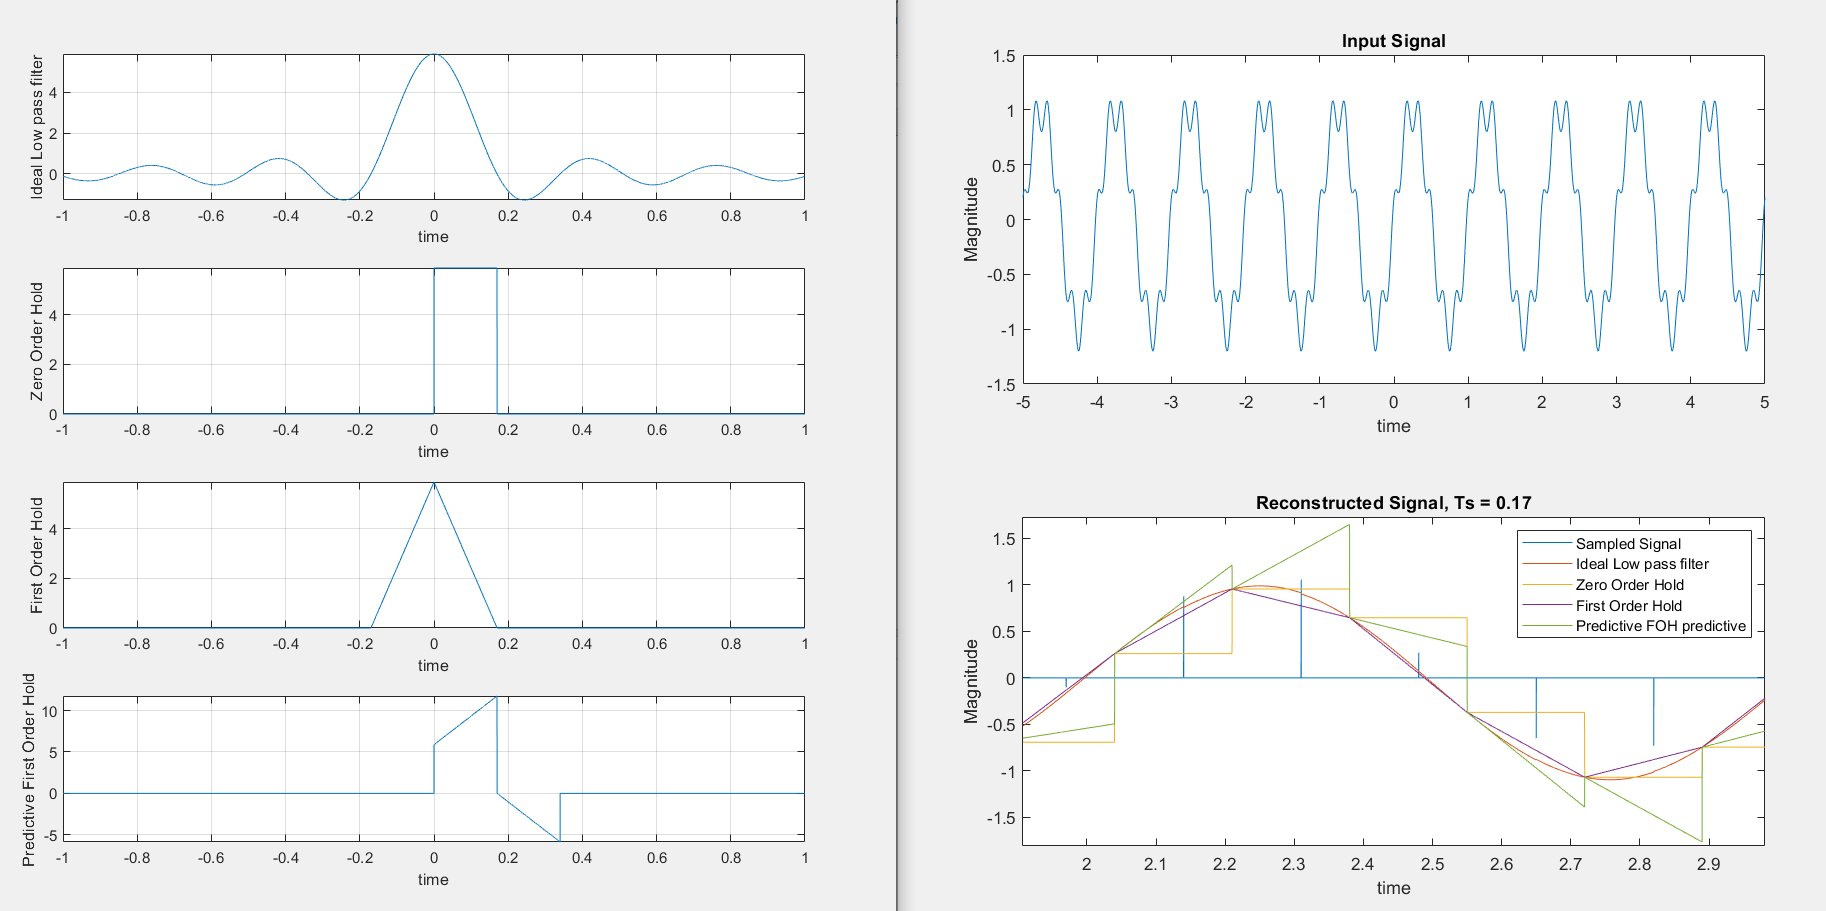
\includegraphics[width=150mm]{figures/Result.PNG}
    \end{center}
    \caption{Reconstruction Closeup}
\end{figure}

\begin{figure}[htbp]
    \begin{center}
	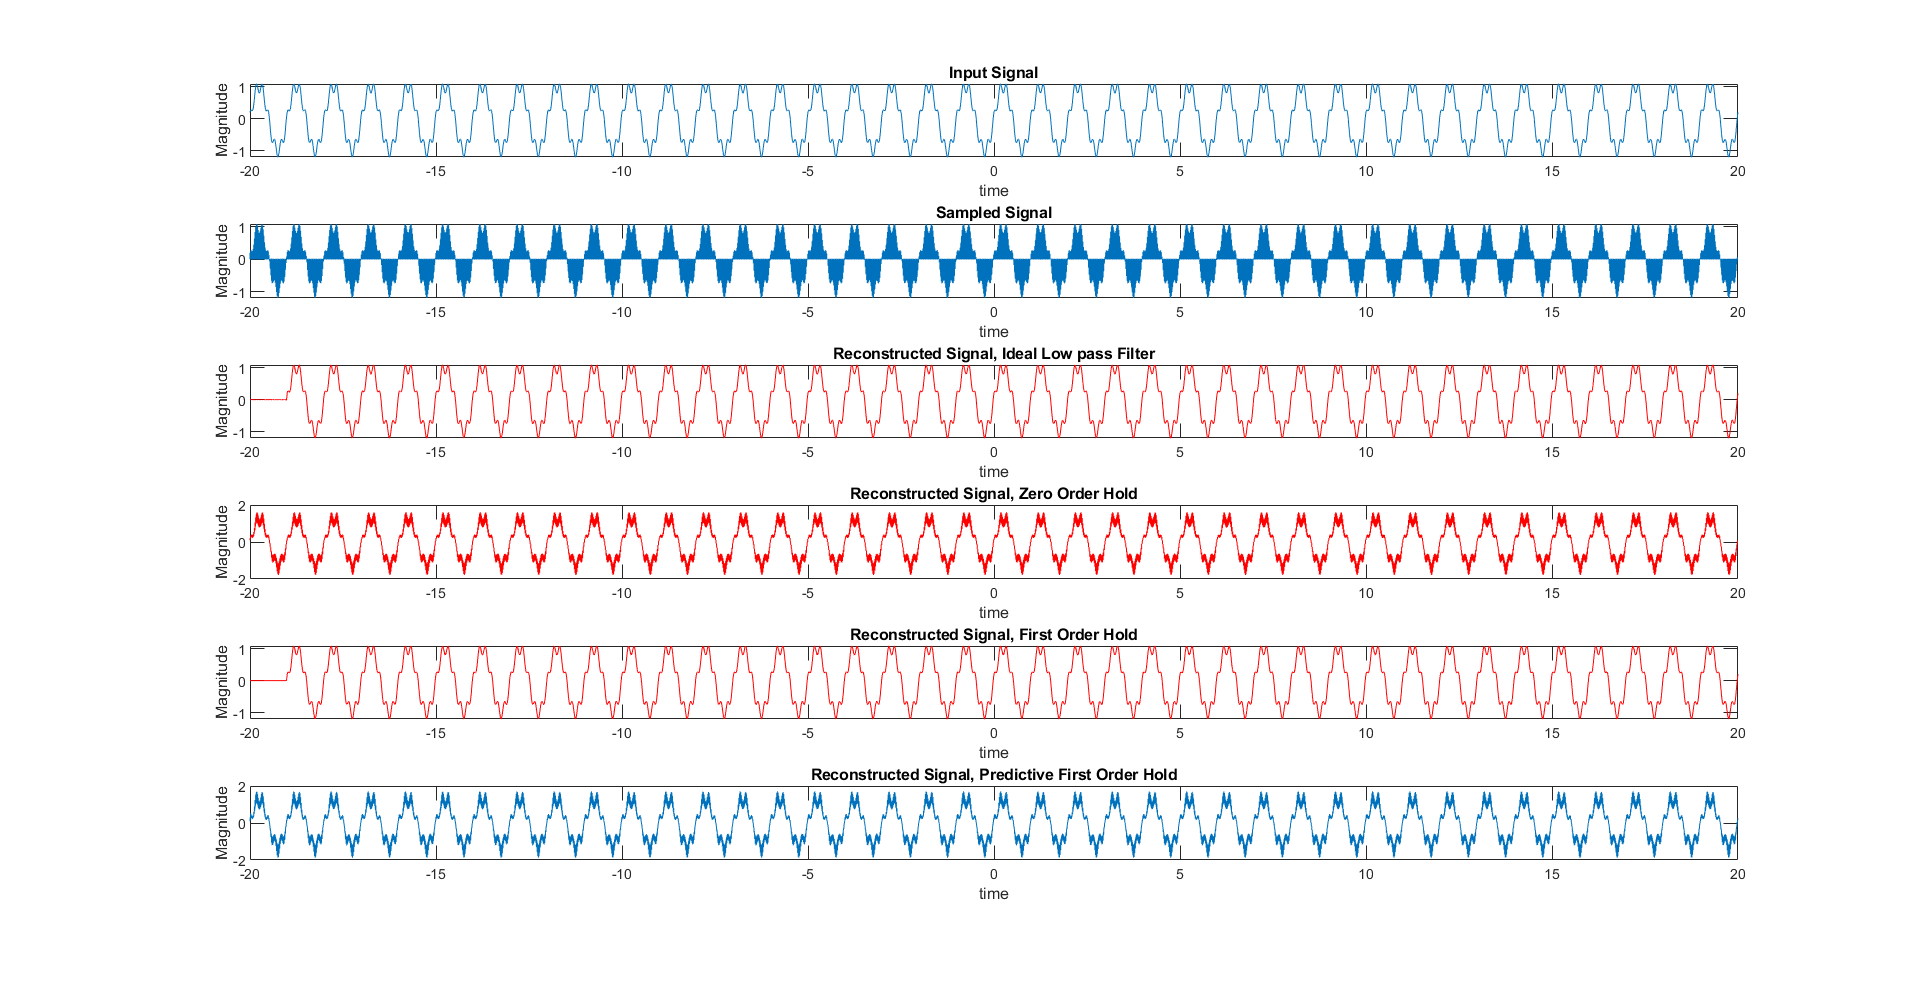
\includegraphics[width=150mm]{figures/Complete_0.017.png}
    \end{center}
    \caption{Reconstruction above Nyquist Shannon Frequency}
\end{figure}

\begin{figure}[htbp]
    \begin{center}
	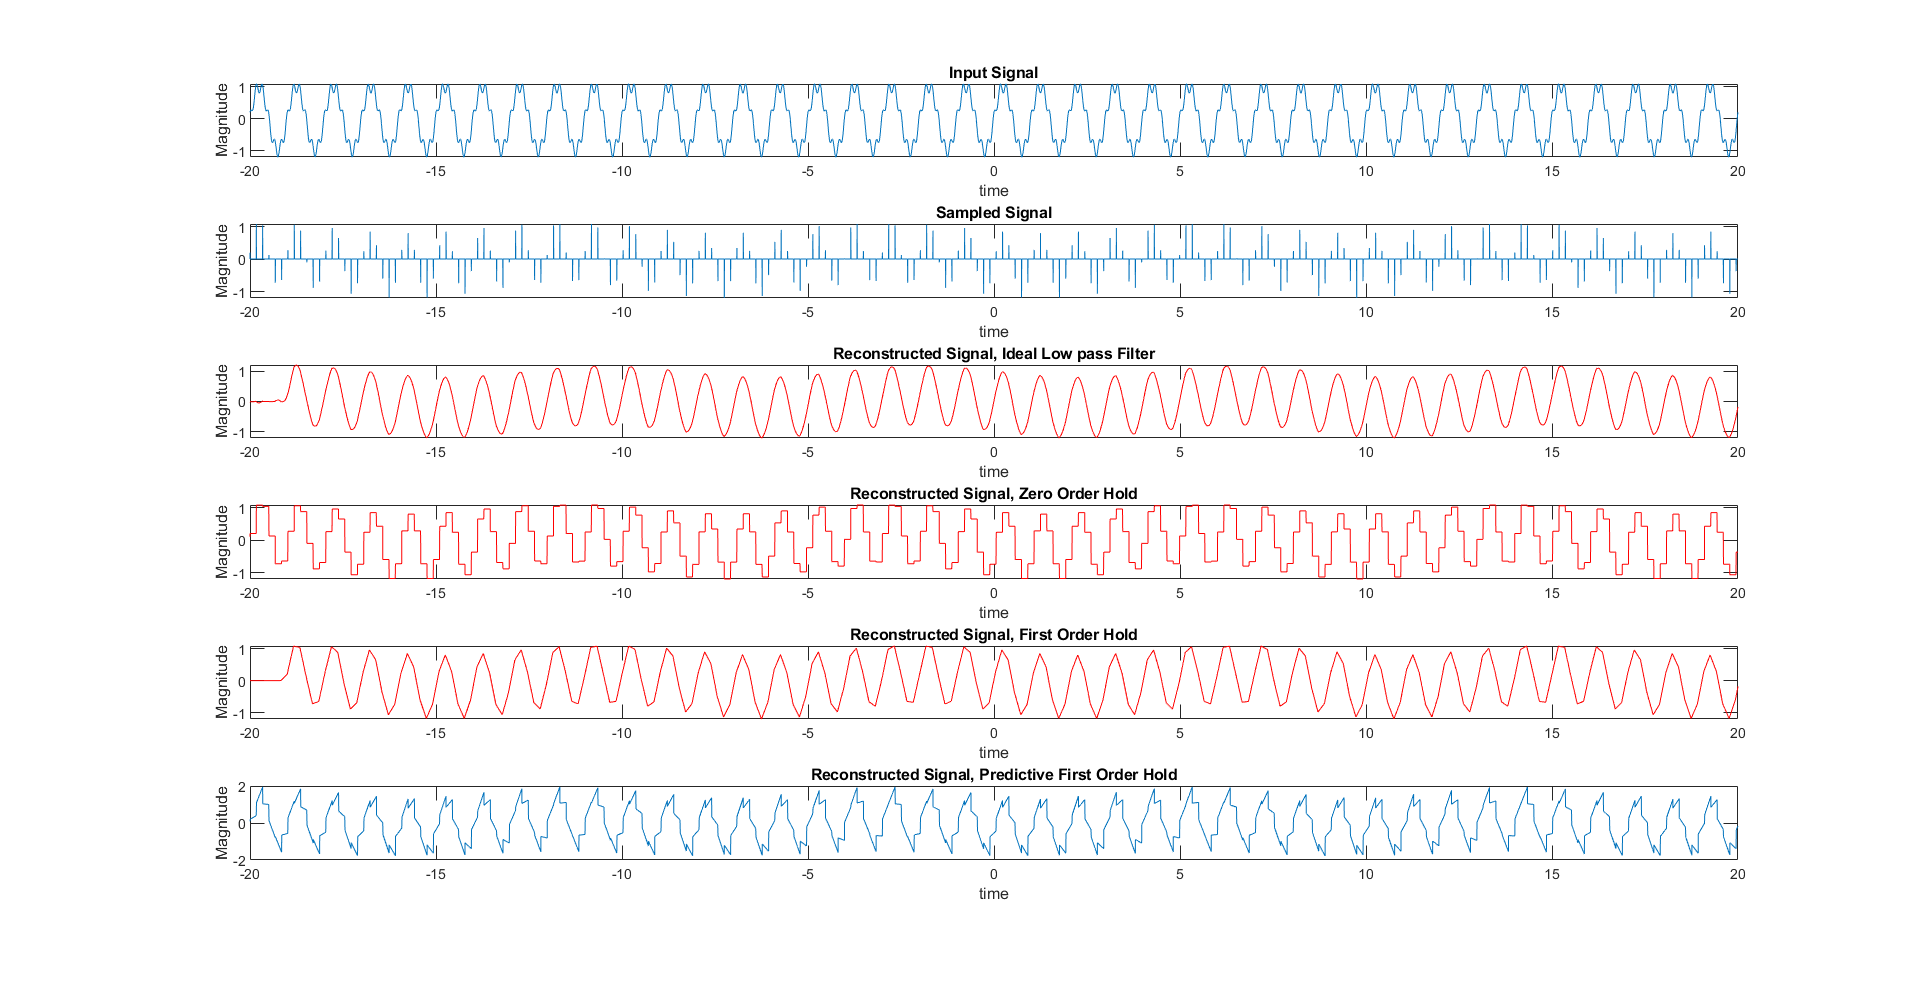
\includegraphics[width=150mm]{figures/Complete_0.17.png}
    \end{center}
    \caption{Reconstruction below Nyquist Shannon Frequency}
\end{figure}
    
    
\begin{thebibliography}{00}
\bibitem{b1} Yang, Chifu et al. “Improving the Closed-Loop Tracking Performance Using the First-Order Hold Sensing Technique with Experiments.” ArXiv abs/1801.01263 (2018): n. pag.

\bibitem{b2} "Signals and Systems - OpenStax CNX." 11 Nov. 2020, cnx.org/contents/d2CEAGW5@15.4:gWKrY9L4@10/Signal-Reconstruction. 

\bibitem{b3} $ Contributors to Wikimedia projects. "Zero-order hold." 8 Mar. 2021, en.wikipedia.org/w/index.php?title=Zero-order_hold&oldid=1010972378. $

\bibitem{b4} "Exp-4 Sampling and signal reconstruction. (Theory) : Signals and Systems Laboratory : Biotechnology and Biomedical Engineering : Amrita Vishwa Vidyapeetham Virtual Lab." 11 Mar. 2021, vlab.amrita.edu/?sub=3&brch=166.

\bibitem{b5} $ https://neuron.eng.wayne.edu/auth/ece4330/lectures/lecture_23_ece4330t.pdf $

\bibitem{b6} Lee, Edward A. and P. Varaiya. “Structure and interpretation of signals and systems.” (2002).

\bibitem{b7} $ "Signals and Systems - OpenStax CNX." 11 Nov. 2020, cnx.org/contents/d2CEAGW5@15.4:IWHZ6hxG@13/Discrete-Time-Processing-of-Continuous-Time-Signals. $

\bibitem{b8} $ Contributors to Wikimedia projects. "Aliasing." 2 Mar. 2021, en.wikipedia.org/w/index.php?title=Aliasing&oldid=1009737665. $

\bibitem{b9} https://www.ni.com/en-us/innovations/white-papers/18/anti-aliasing-filters-and-their-usage-explained.html

\bibitem{b10} Zheng Zhang and Kil To Chong, "Comparison between first-order hold with zero-order hold in discretization of input-delay nonlinear systems," 2007 International Conference on Control, Automation and Systems, Seoul, Korea (South), 2007, pp. 2892-2896, doi: 10.1109/ICCAS.2007.4406863.

\end{thebibliography}


\appendix
\begin{appendices}
    \begin{enumerate}
        
        \item All the codes for used in this project is available at this repository at \\ \textbf{https://github.com/arpit6232/Industrial-Automation} 
    \end{enumerate}
\end{appendices}

\end{document}
